\chapter{Synthesizing Data for the Detection of \ac{EWFO} on \acp{MAV}}

This chapter addresses the generation of data for the detection of \ac{EWFO}. In particular the following research question is addressed:\\
\begin{centering}
\textbf{How can data be generated to train a detection model for \ac{EWFO} detection on a \acp{MAV}?}
\end{centering}

The question is subdivided in three research questions to be addressed in this chapter:
\begin{enumerate}
	\item[\textbf{RQ1.1}] What role does context play for the detection \acp{EWFO} on \acp{MAV}?
	\item[\textbf{RQ1.2}] What role does the view perspective play for the detection \acp{EWFO} on \acp{MAV}?
	\item[\textbf{RQ1.3}] Can the incorporation of sensor effects or image augmentation benefit the detection performance?
\end{enumerate}

The chapter starts by introducing terminology and the data generation pipeline. In the later sections each research question is addressed in several experiments. The chapter finishes with an overall conclusion.

\section{Methodology}
\label{sec:datagen:method}
\begin{figure}[htbp]
	\centering
	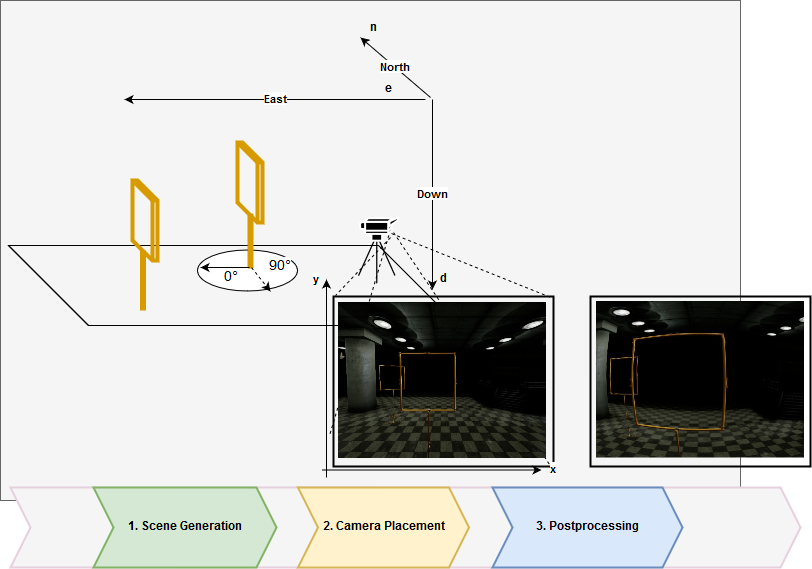
\includegraphics[width=0.9\textwidth]{fig/datagen_notation}
	\caption{Overview of the data generation process.}
	\label{fig:training:datagen_notation}
\end{figure}

A data generation pipeline is implemented using OpenGL, UnrealEngine and AirSim. An overview can be seen in \Cref{fig:training:datagen_notation}. In the first step a scene is created in which the objects of interest as well as the camera are placed. In 3D space position and orientation (pose) of each object are determined by translation $\textbf{t}$ and rotation $\textbf{r}$. The coordinate system is \ac{NED}.

A view projection yields an image through the lens of the camera. The coordinates of each point in 3D space are projected on the 2D image plane. A final post processing step can simulate further effects like lens distortion and sensor noise. This step is implemented using OpenCV and Python. All source code is made publicly available at \url{https://github.com/phildue/datagen.git}.

Within the pipeline environments for training and testing are created. A black environment serves as base to replace the background with existing images. Furthermore, three indoor base environments are created that fully simulate illumination and background. An overview can be seen in \Cref{fig:environments}. Within the environment light conditions, background textures, object locations can be changed manually. The environments are described in the following:

\begin{enumerate}
	\item \textit{Dark:} The environment is a room without windows, only containing artificial light sources. 
	\item \textit{Daylight:} The environment is a room with windows along all walls that allow daylight to illuminate the room. The windows can lead to strong variations in the contrast between different parts of the object.
	\item \textit{IROS:} The environment resembles the room of the \ac{IROS} Autonomous Drone Race 2018. The light sources stem from a window front at one side of the room, as well as artificial light sources at the ceiling. Depending on the view point, the object might appear against bright or dark background.
\end{enumerate}

\begin{figure}[hbtp]
	\centering
	\begin{minipage}{0.3\textwidth}
		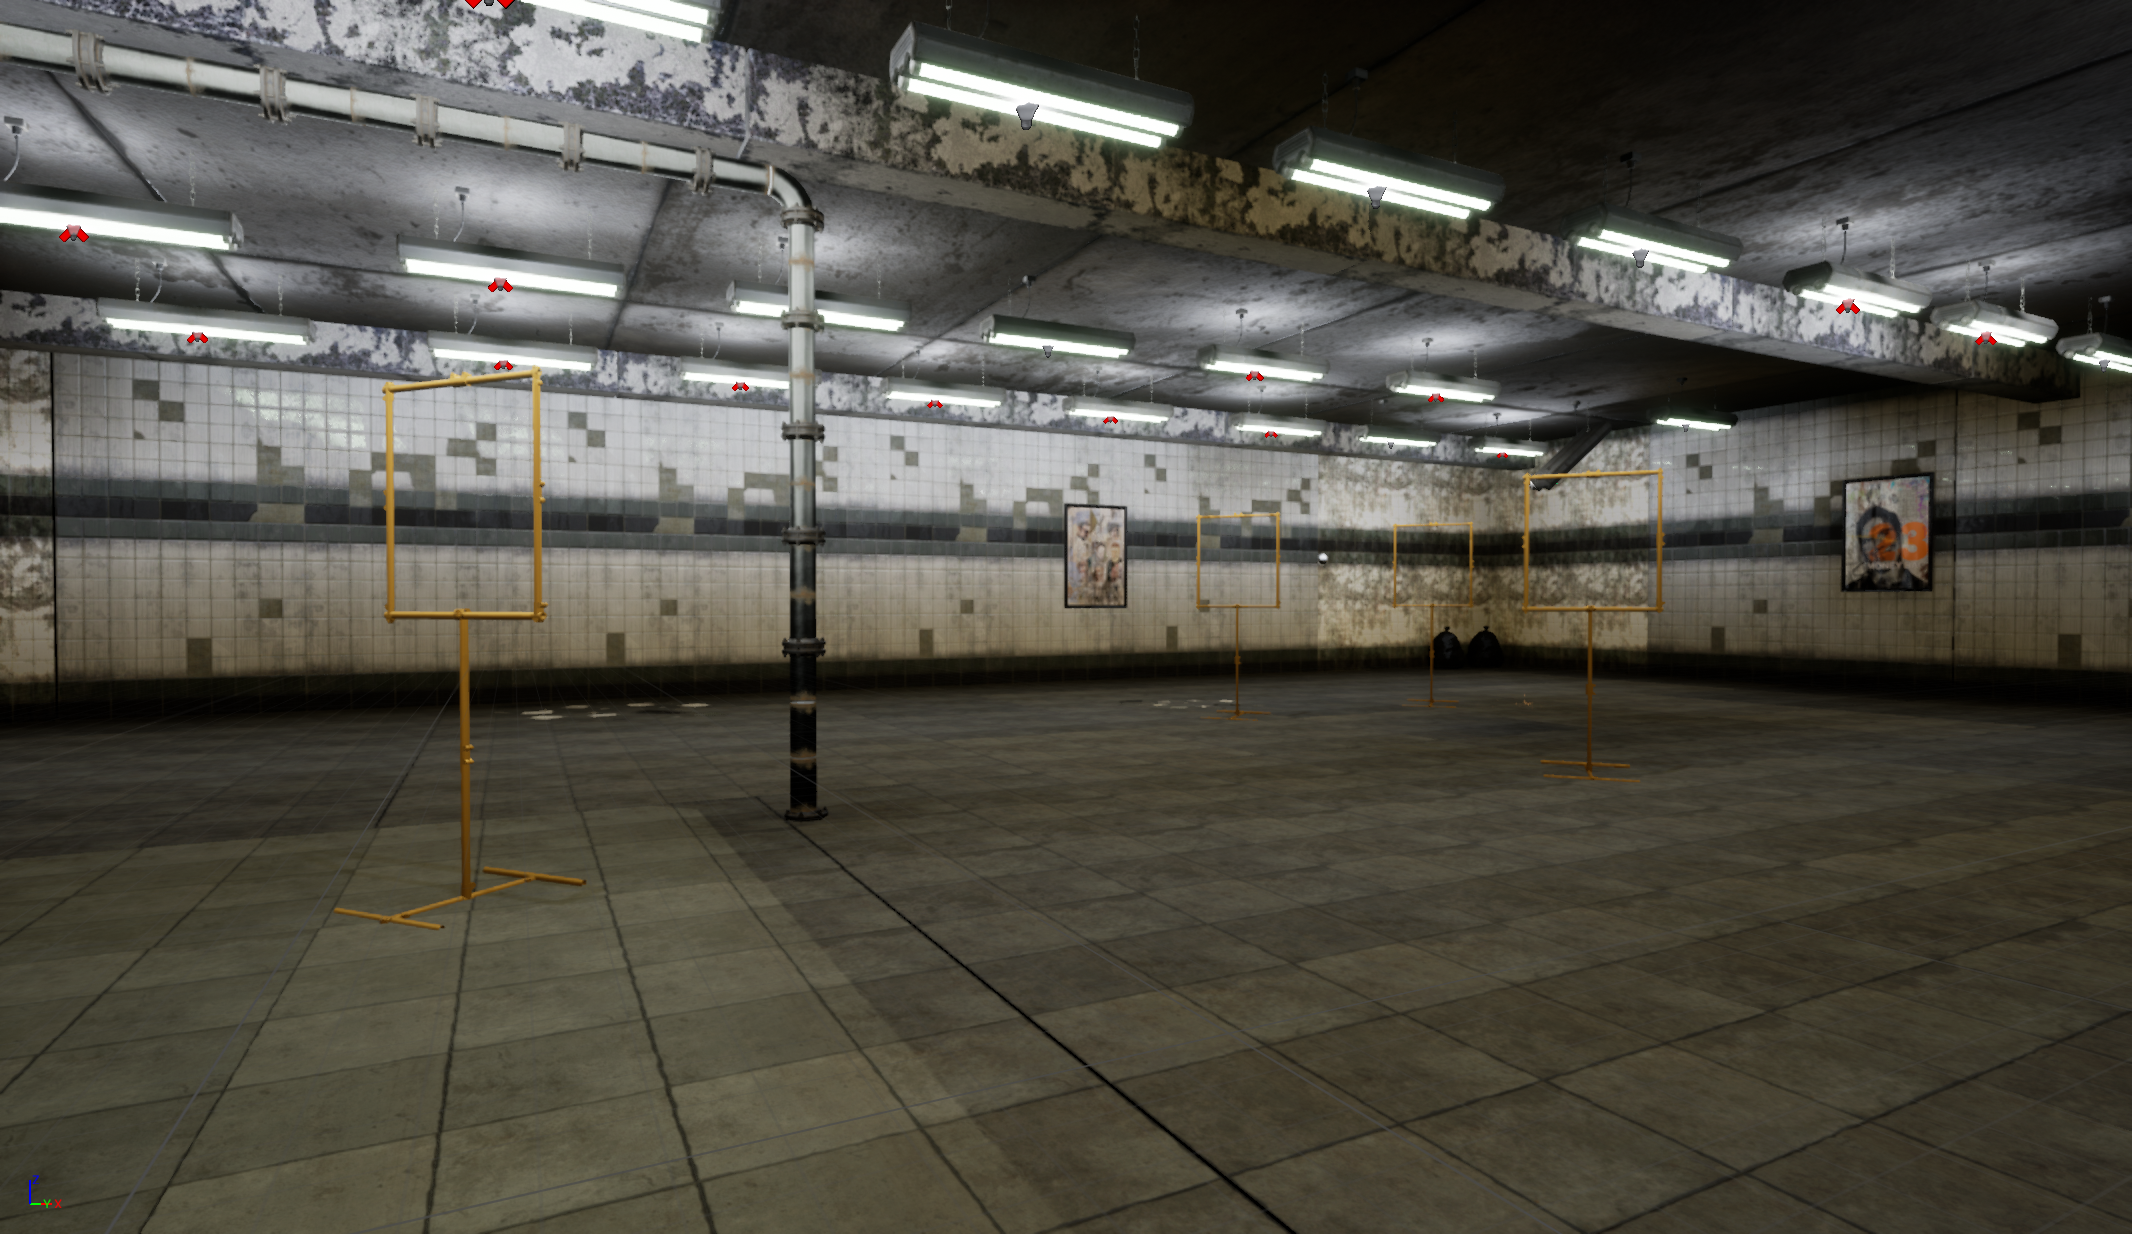
\includegraphics[width=\textwidth]{fig/basement_perspective}
	\end{minipage}
	\begin{minipage}{0.3\textwidth}
		\includegraphics[width=\textwidth]{fig/daylight_perspective}
	\end{minipage}
	\begin{minipage}{0.3\textwidth}
		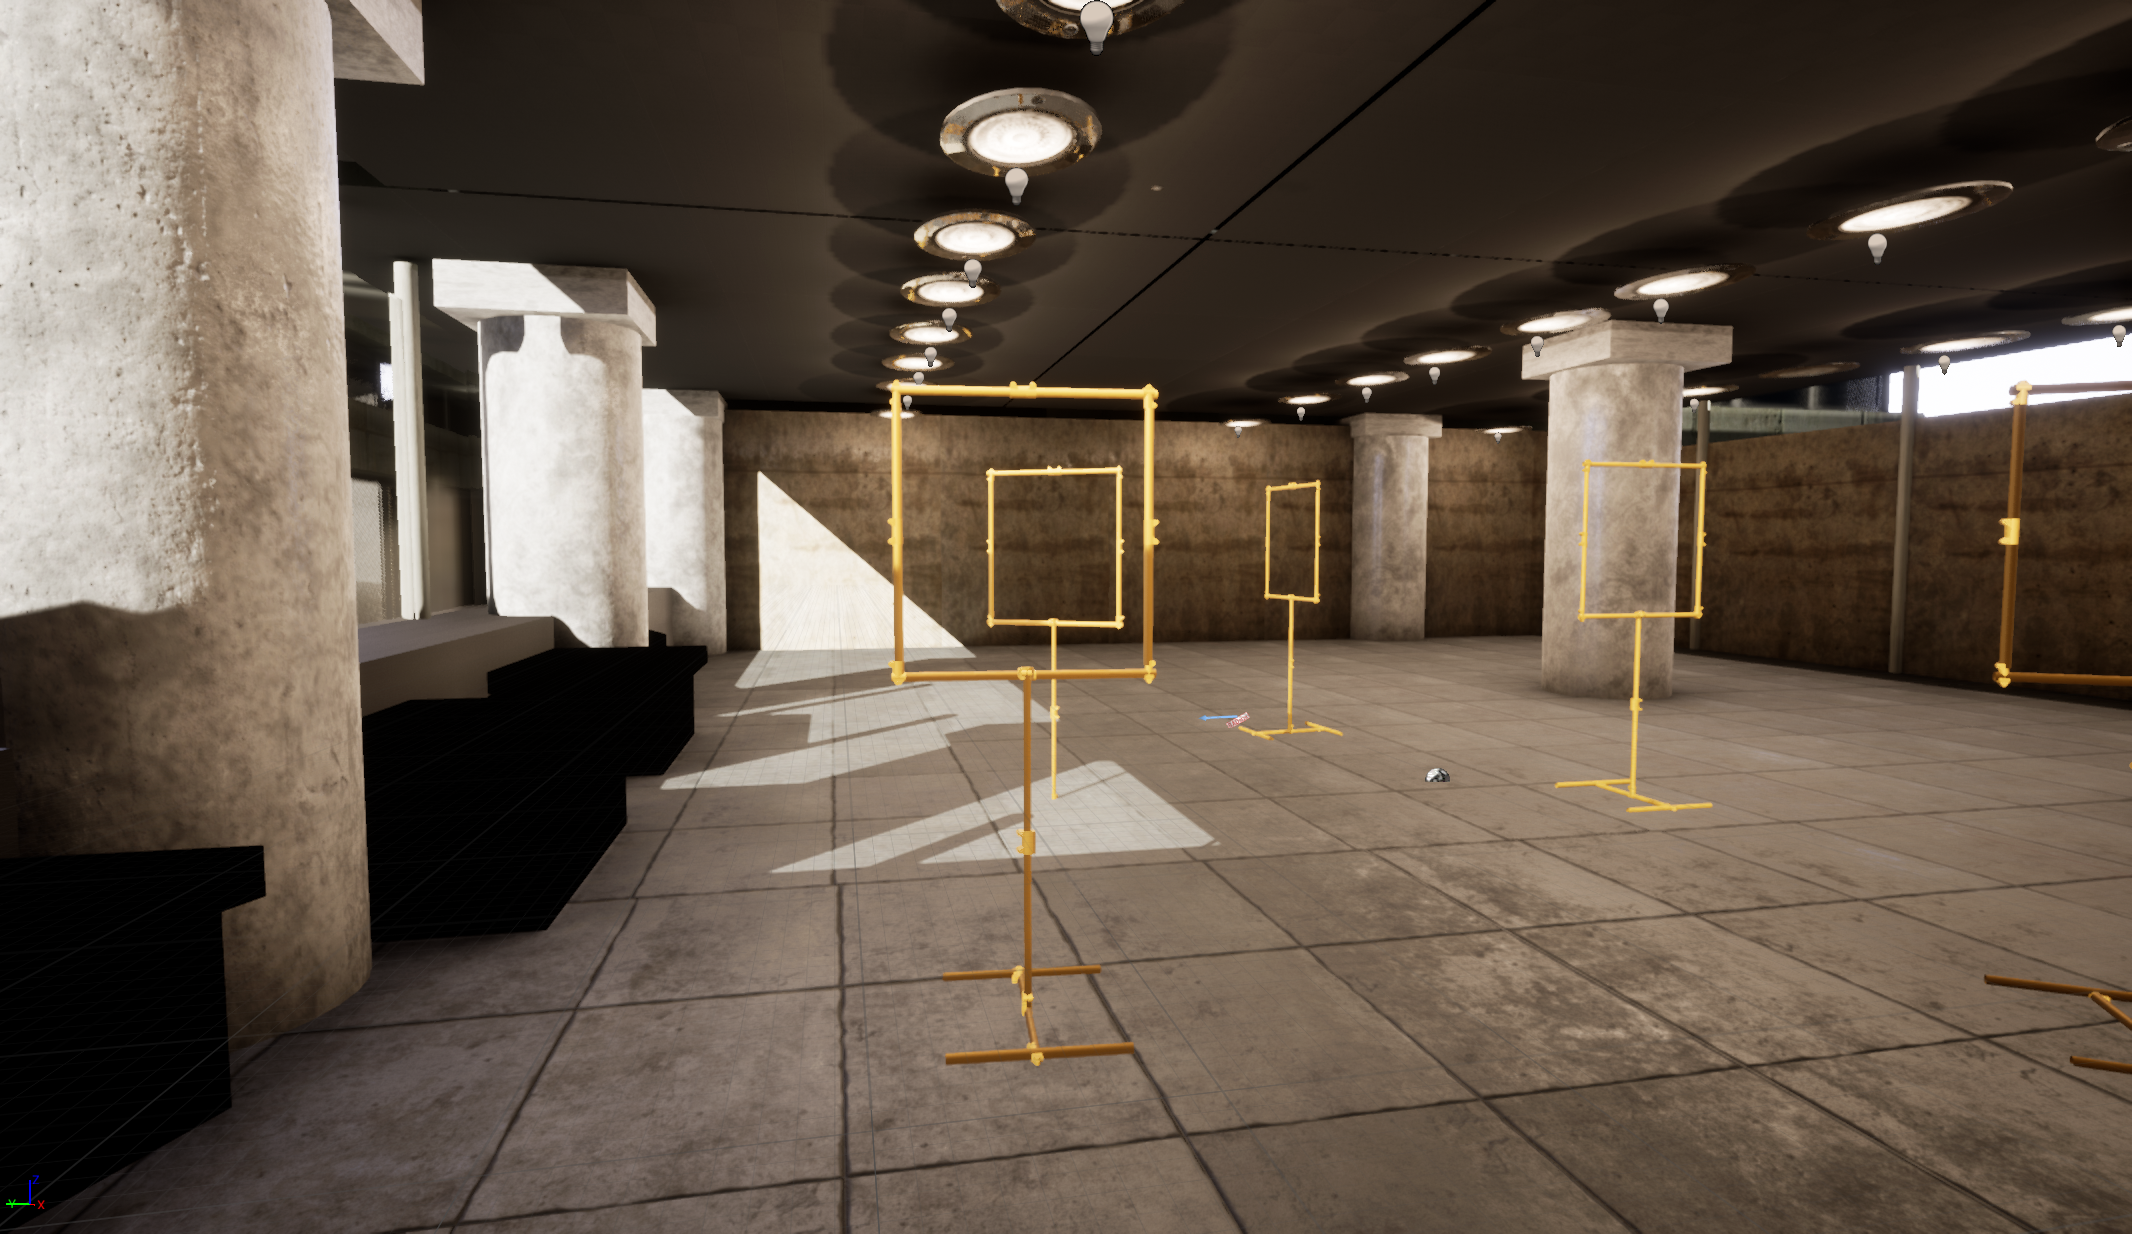
\includegraphics[width=\textwidth]{fig/iros_perspective}
	\end{minipage}
	\caption{The environments from left to right \textit{Dark}, \textit{Daylight}, \textit{IROS2018}}
	\label{fig:environments}
\end{figure}

The data generation pipeline is used to generate a test set in simulation. The test set is set up in the \textit{IROS} environment and inspired by the race court of the \ac{IROS} Autonomous Drone Race. The AirSim flight controller is used to simulate a flight of an \ac{MAV} through the race court. The test set contains 550 images with a total of 1361 objects.

It should be noted that when generating data with the described methods it is likely that samples appear in which only a corner of the object is visible or the view angle is in such a way that the object appears only as a thin line. In initial experiments these corner cases led to unstable training. Hence, some minimum requirements for the labels are set and samples/labels are removed if these are not met. Objects have to have a minimum size of 1\% of the image area as well as an aspect ratio between 1/3 and 3/1. Furthermore, at least three corners have to be visible.

The models and training are implemented using the \textit{Keras} framework with \textit{tensorflow}-backend. For all trainings the Adam optimizer is applied using a learning rate of 0.001 for the first 60 epochs and a learning rate 0.0001 afterwards. A validation set containing 1\% randomly sampled images from the training set is used. The training is stopped if the validation error does not decrease for more than 5 epochs or 100 epochs are reached.

Throughout the experiments the baseline TinyYoloV3 architecture is used. Thereby we simplify the loss function to a single class prediction. The exact model is described in \Cref{sec:object_detection}. The input image resolution is 416x416.

\section{Context}

The context in which an object is placed consists of background as well as light conditions or other objects. It is determined in the first step of the data generation process. Theoretically \acp{CNN} can learn to exploit context for detection. Yet, the actual influence is not clear. For example the Object Detectors trained in \cite{Peng} do not seem to make use of this image cue. Nevertheless, we investigate the importance of context for the detection of \acp{EWFO}. We hypothesize that due to the sparsity of their features and their emptiness context and background plays a more important role than for solid objects.

For the investigation we compare three methods to generate data: The placement of \ac{CAD}-models on uniformly coloured backgrounds, on backgrounds taken from a dataset as well as from fully synthesized environments. In terms of geometric and physical properties the fully synthesized environments provide the most realism and hence should give the best results. However, as the graphical engine only contains a limited set of textures, the variance in background is way smaller than in the backgrounds taken from a dataset. Furthermore, the objects in the background are also rendered. Hence, when tested on real data this method could lead to better performance.

\subsection{Experiments}

Four datasets are generated with 20 000 samples each. Dataset I contains samples generated by placing \ac{CAD}-models on uniformly coloured backgrounds; Dataset II contains samples generated by placing \ac{CAD}-models on backgrounds taken from the Pascal VOC dataset, Dataset III contains samples from the \textit{Dark} environment, Dataset III contains samples from all virtual environments. A fourth model is trained on a combination of Dataset II and IV (equal proportion).

Within the environment the camera is placed at random locations following these distributions:

\begin{equation}
x = \mathcal{U}(-30,30),\quad y = \mathcal{U}(-20,20),\quad z = \mathcal{N}(-4.5,0.5)),\quad
\phi = \mathcal{U}(0,0.1\pi),\quad \theta = \mathcal{U}(0,0.1\pi),\quad \psi = \mathcal{N}(-\pi,\pi)
\label{eq:distroexp}
\end{equation}

Where $ \mathcal{U}(a,b)$ is a uniform distribution between $a,b$ and $\mathcal{N}(\mu,\sigma^2)$ is a Gaussian distribution with mean $\mu$ and variance $\sigma^2$.

The models are tested on the real datasets described in \Cref{sec:datasets} as well as the simulated flight described in \Cref{sec:datagen:method}.


\subsection{Results}

\Cref{fig:context} display the results. It can be seen how using uniformly coloured backgrounds achieve almost no detection. Only on the simulated data a few objects could be detected.

In contrast using fully synthesized data achieves the best performance on the simulated data for low and high quality detections. It can be seen that almost all detections have an \ac{IoU} of more than 60\% and are thus good quality. On the real data the performance in low quality detections is comparable to the performance on the simulated data. However, in hiqh quality detections the performance drops significantly to an equal level of using real backgrounds.

Using real backgrounds performs poorer than using a fully synthesized environment in almost every case. However, for higher quality detections the performance is competitive to using a fully synthesized environment. Combining both methods does achieve at most the performance of using fully synthesized data. However, in most cases the performance is worse.   

\if false
\begin{table}[htbp]
	\caption{Results of different ways to generate context.}
\begin{tabular}{lrrrrrr}
	\hline
	Name &  Sim Data0.4 &  Sim Data0.6 &  Sim Data0.8 &  Real Data0.4 &  Real Data0.6 &  Real Data0.8 \\
	\hline
      Real Backgrounds &         0.26 &         0.15 &         0.02 &          0.14 &          0.09 &          0.01 \\
  Uniform Backgrounds &         0.04 &         0.02 &         0.00 &          0.00 &          0.00 &          0.00 \\
  Various Environments &         0.32 &         0.31 &         0.08 &          0.33 &          0.10 &          0.01 \\
        Real + Various &         0.32 &         0.18 &         0.04 &          0.12 &          0.10 &          0.01 \\
\hline
\end{tabular}
	\label{tab:context}
\end{table}
\fi
\begin{figure}[htbp]
	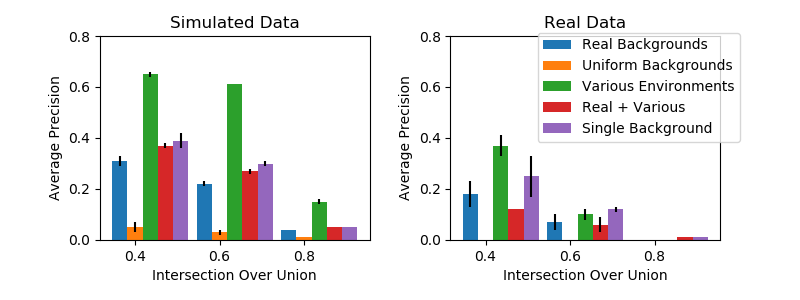
\includegraphics[width=\textwidth]{fig/context_bar}
	\caption{Results of different ways to generate context. Synthesizing more parts of the environment improves performance on both test sets. However, this only holds for weakly localized predictions.}
	\label{fig:context}
\end{figure}

\subsection{Discussion}

The results meet our hypothesis that using only uniformly coloured backgrounds is not enough to train an Object Detector for \ac{EWFO}. Providing more variance in the background is crucial to improve performance.

Despite having not seen a single real background, the model trained on fully synthesized data achieves the best performance on the real data. Even a model trained in a single virtual environment achieves competitive performance. Hence, it seems that synthesizing correct geometric/physical properties is more important than providing a large variance in background. However, the margin gets small for higher quality detections. Thus, the simulation of geometric/physical properties does not help for good localization.

\subsection{Conclusion}

We investigated the role context plays for the detection of \acp{EWFO} on \acp{MAV}. We can conclude that providing some background is crucial for the detection. Otherwise the detector performs poorly in simulation as well as the real world. Furthermore, synthesizing the whole environment benefits the detection on real images. However, most of the additional detections have not very accurate bounding boxes.

\section{View}

Another important property that influences the generated sample is the camera pose. It determines the view on the scene and therefore at which distance, angle and location the objects appear on the image.

A straightforward way is placing the camera randomly (within some margin) in order to cover a large variation of views on the object. That way the network can learn a general object representation and hopefully detect unseen objects from different view points. However, random  placement might not resemble the real world sufficiently. An \ac{MAV} does not appear at random places within a scene, especially not when it follows a racing track. We examine this by simulating a flight through a race court using AirSim's \ac{MAV} model and analyzing the relative object poses. We compare these to the relative poses obtained when placing the camera randomly using the distributions from \Cref{eq:distroexp}.

\begin{figure}
	\begin{minipage}{\textwidth}
		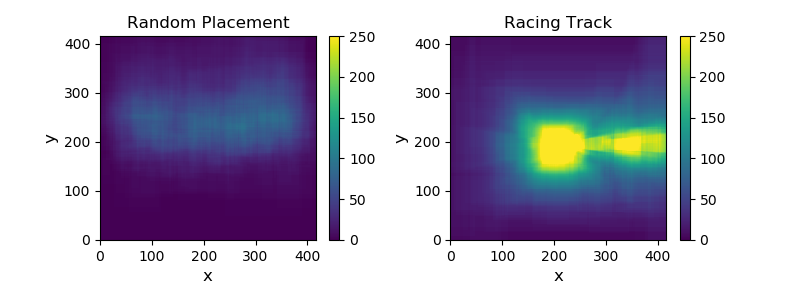
\includegraphics[width=\textwidth]{fig/heatmap_camplace}
		\caption{Object appearances when generating samples with random poses (left) and during a \ac{MAV} flight. During the flight the object appears mostly centered on the horizontal line.}
		\label{fig:heatmap_camplace}
	\end{minipage}
	\begin{minipage}{\textwidth}
		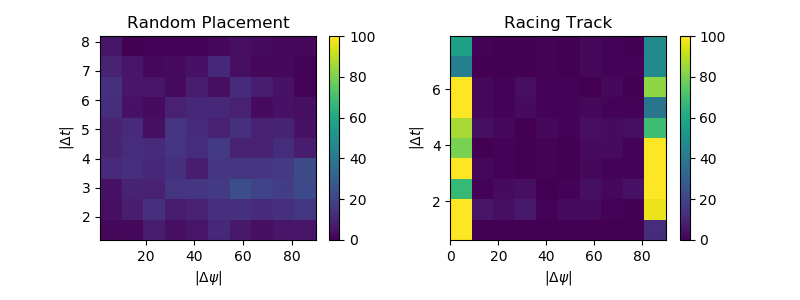
\includegraphics[width=\textwidth]{fig/hist2d_camplace}
		\caption{Histogram of object occurrences in yaw angle and distance relative to the camera. The random placement does rarely cover facing the object closely and frontally. }
		\label{fig:hist2d_camplace}
	\end{minipage}
\end{figure}

\Cref{fig:heatmap_camplace} shows the distribution of bounding boxes when created with random camera placement and when following a racing track. It can be seen how, when following the race track most of the objects are centered and distributed across the horizon, as camera focuses the next object frontally most of the time. In contrast, random placement leads to more evenly distributed object locations. This can also be seen in \Cref{fig:hist2d_camplace} where a 2D histogram of the yaw angle and distance with respect to the camera is displayed. Thereby 0 corresponds to facing the object frontally, 180 degrees facing the object from the back. It is apparent how the random placement covers a much larger range of relative angles, while in the racing track certain angles do not appear at all. Even more importantly the largest bins of the racing track is an angle of 0 and a distance between 0m and 4m. These bins are almost not present when placing the camera randomly. This is because close to the camera the field of view is small, while the area of the object faced frontally is big. Hence, the probability of an object ending up at this specific location is relatively low. Furthermore, when placing the camera randomly there are no samples further away than 8m. This is because in the race track the camera traverses the room from one end - where it can see almost all gates - to another. The probability that the randomly placed camera ends up in a similar position is relatively low.

The filters of \acp{CNN} are translation invariant by design but cannot inherently handle variation in rotation and scale. We hypothesize that the generation of samples with only one of the two methods can miss important object appearances. Random placement does not cover appearances that are typical for a autonomous drone race. On the other hand, only training on racing tracks might lead to a bias towards the created courses.

\subsection{Experiments}

In order to to evaluate this hypothesis three models are trained on 20 000 samples each. Model I is trained when placing the camera randomly, following the distribution in \Cref{eq:distroexp}. Model II is trained on varying racing courts. Model III is trained on a combination of both datasets (equal proportion).

The models are tested on the real datasets described in \Cref{sec:datasets} as well as the simulated flight described in \Cref{sec:datagen:method}.

\subsection{Results}

\begin{figure}[htbp]
	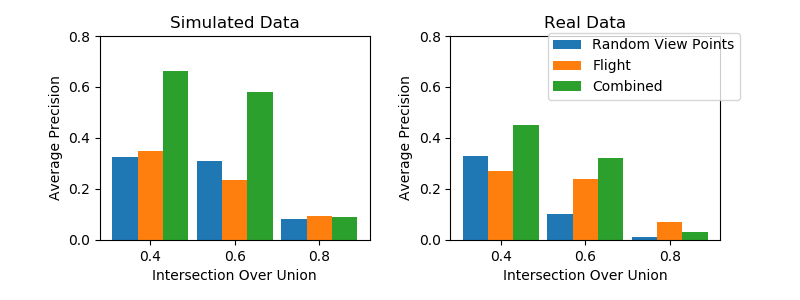
\includegraphics[width=\textwidth]{fig/view_bar}
	\caption{Average Precision for the three different models.}
	\label{fig:view_bar}
\end{figure}

\Cref{fig:view_bar} shows the average precision of the different models. It should be noted that \textit{Random View Points} is the same model as \textit{Various Environments} of \Cref{fig:context}. On the simulated dataset there is only a minor difference between the three models in terms of average precision. In contrast on the real world dataset it can be seen how the models that include flight images perform better for higher quality detections. The best performance is achieved by the model that was trained on a combination of both datasets.

\begin{figure}[htbp]
	\centering
	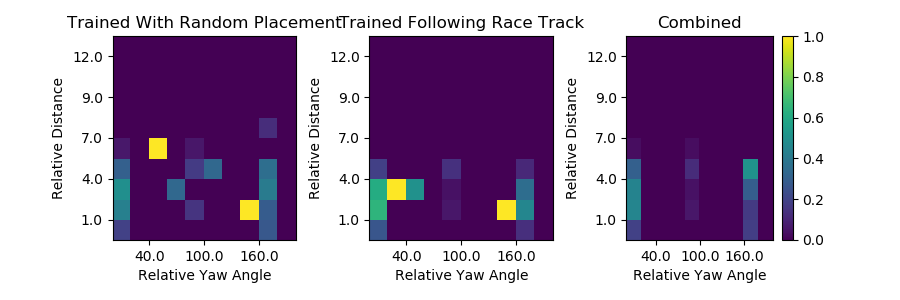
\includegraphics[width=\textwidth]{fig/recall_yaw}
	\caption{Recall on clusters depending on yaw angle and distance.}
	\label{fig:recall_yaw}
\end{figure}

\Cref{fig:recall_yaw} shows the performance of the different models in terms of recall on the simulated dataset at a confidence threshold of 0.5. It can be seen that the recall of the model only trained on racing tracks is lower than the recall of the other models. This holds particularly when the object is not faced frontally. Between the combined dataset and random placement only minor differences can be identified.

Despite the lower recall the model trained on racing tracks achieves comparable performance in terms of AP. This is explained by the higher precision achieved by the model.

\begin{figure}[htbp]
	\centering
	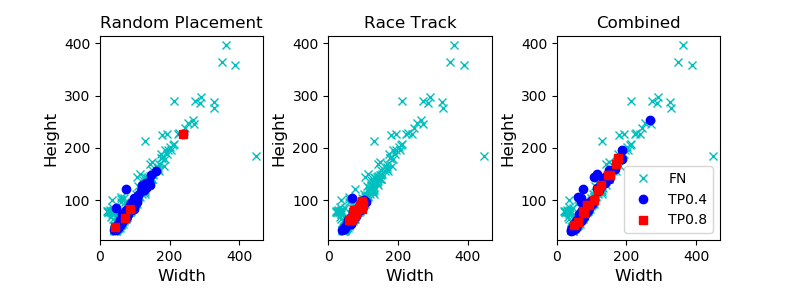
\includegraphics[width=\textwidth]{fig/view_scatter}
	\caption{Detections on the real data shown with respect to width and height of the bounding box. The more top left a sample is located the closer it is to the camera. When Height > Width the object mostly has a yaw angle unequal to zero.}
	\label{fig:view_scatter}
\end{figure}

\Cref{fig:view_scatter} shows true positives at different \ac{IoU} thresholds as well as false negatives of the real data. It can be seen how the models that cover more relative view angles in their training data have a broader range of detections. The model trained on racing tracks only detects objects at quite narrow field. It is also apparent how the model trained on a combination of both datasets not only detects the same objects as the other two models but also objects.

On the real as well as on the simulated data it can be seen that there is some distance were the model performs best. Objects that are very close or too far are not detected by any of the models.

\subsection{Discussion}

Even though one model is trained on various race courts, containing many samples with objects close to the camera there is no significant performance increase for those samples. Instead this model produces higher quality bounding boxes while overall detecting less objects. The model trained on random view points seems to detect more objects but the predicted bounding boxes are poorer. Hence, there seems to be a trade-off between detecting angles at more view points and the quality of the respected bounding boxes. 

It can also be seen that the combined model learns to detect not only the same objects as the individual models but also totally new objects. Hence, it can be assumed covering more angles in the training set helps to generalize. 

It can also be observed that the performance for objects that are close to the camera are quite poor for all models. This is potentially explained by the fact that less object context is available. For example the pole for closer objects is less visible. Also, the probability of having a part of the object out of view increases as the camera comes closer. Another issue could be the limited receptive field of the detection model. As the last node of the model cannot see the whole image and the object is empty, it is possible that the node responsible to predict the object does not see any of the object parts. This is further addressed in \Cref{sec:object_detection}.

For larger distances the performance decreases again. This is explained by the fact that less details of the objects are visible as the camera moves further away.

\subsection{Conclusion}

We investigated the influence of the relative view for the detection of \ac{EWFO} on \ac{MAV}. We hypothesized that having a higher variance in view points will improve the detection and that including samples obtained from racing tracks is crucial for detecting close objects. However, we could not observe a direct relation between the view angles present during training and the model performance on different angles. Instead we observe that the model containing less angles in the training set produces less but higher quality bounding boxes. Furthermore, we observe that including the racing track images helps the model to generalize and improves performance on the real world dataset.

\section{Image Augmentation}

The final step applies low-level image transformations. It allows to further simulate sensor effects and increase the variance in the generated data.

In literature \cite{Krizhevsky2012a,Howard2013,Redmon,Liu} the application of image augmentation is a common tool to improve the detection performance. The experiments in \cite{Carlson2018} show how the incorporation of sensor effects particularly improves the performance of models learned on fully synthesized data. In the \ac{MAV} domain sensor and lens effects have a significant influence on the obtained sample. Hence, we hypothesize that the incorporation of these effects will improve the performance of the trained models. A total of  five image augmentation techniques are investigated.

\paragraph{Lens Distortion}

Lens distortion is a form of optical aberration which causes light to not fall in a single point but a region of space. For \acp{MAV} commonly used wide-angle lenses, this leads to barrel distortion and thus to straight lines appearing as curves in the image.

For this work a 120 wide angle lens is used. Especially, close objects undergo a strong variation in appearance. Hence, we hypothesize including this effect in the training process will improve the performance on the real world dataset. 

The effect is applied using the model for wide-angle lenses from \cite{Vass}. It models the removal of lens distortion as combination of radial and non-radial part, that is approximated with a second order Taylor expansion:
\todo{double check formula is (y in first line?)}
\begin{equation}
\begin{pmatrix}
x_u \\
y_u  
\end{pmatrix}=
f(x,y) =
\begin{pmatrix}
x (1 + \kappa_1 x^2 + \kappa_1 (1 + \lambda_x) y^2 + \kappa_2(x^2 + y^2)^2) \\
y (1 + \kappa_1 x^2 + \kappa_1 (1 + \lambda_y) y^2 + \kappa_2(x^2 + y^2)^2)
\end{pmatrix} 
\label{eq:distortion}
\end{equation}
Where:
\begin{itemize}
	\item $x_u$ and $y_u$ are the undistorted coordinates.
	\item $\kappa_1$ $\kappa_2$ control the radial distortion 
	\item $\lambda_x$ and $\lambda_y$ control the tangential distortion
\end{itemize}

Applying the lens distortion to an image is done using the inverse of \Cref{eq:distortion}. However, as there is no closed form solution, so the Newton-approximation.

An example with $\kappa_1 = 0.5, \kappa_2 = 0.5$ is displayed in \Cref{fig:distortion}. It can be seen how the previously straight lines appear as circular shape.

\paragraph{Chromatic Aberration.}

Chromatic Aberration is caused when different wavelengths of light do not end up in the same locations of the visual sensor. This leads to a shift in the colour channels of the image.

In \cite{Carlson2018} including chromatic aberration significantly improves the performance of models that are trained on fully synthesized data. Hence, we hypothesizes this will also help for our work.

Similarly to \cite{Carlson2018}, chromatic aberration is applied by scaling the locations of the green channel, as well as applying translations on all channels. The model can be implemented as affine transformation of the pixel locations for each channel:

\begin{equation}
f(x_C,y_C) = \begin{pmatrix}
S & 0 & t_x \\
0 & S & t_y \\
0 & 0 & 1
\end{pmatrix} \begin{pmatrix}
x_C \\
y_C \\
1
\end{pmatrix}
\end{equation}

Where $C$ is one colour channel of the image.

An example is displayed in \Cref{fig:chromatic}. It can be seen how the red and green channel are shifted relative to each other. Thus two bars appear in the image.

\paragraph{Blur}

Fast movement and sensor noise can lead to blurry images. This is particularly present in the domain of \ac{MAV}/Autonomous Drone Racing. Hence, we hypothesize including this effect will improve the detection in the real world. 

The effect is modelled using a Gaussian-filter. The image is convolved with a 2D-kernel build from:

\begin{equation}
k(x,y) = \frac{1}{2\sigma_x\sigma_y\pi}e^{-\frac{1}{2}({\frac{(x-\mu_x)^2}{\sigma_x^2} + \frac{(y-\mu_y)^2}{\sigma_y^2}})}
\end{equation}

Where $\sigma_x$ and $\sigma_y$ are the variance in direction x and y, used to model directional (motion) blur and $\mu_x$, $\mu_y$ are at the kernel center. An example can be seen in \Cref{fig:focusblur}.

\paragraph{Exposure.}

Exposure is the time the sensor records light in order to create an image. Over- and Underexposure are caused when this time is too short or too long, leading to too dark or too bright images.

Cameras typically have Autoexposure-functionality which adapts the exposure time depending on light conditions. However, the adoption is not instant, sudden light changes can lead to over- or underexposure. This particularly applies during a fast flight. Hence, we hypothesize incorporating the effect in the data generation will improve the performance of the trained model. The effect is modelled following \cite{Carlson2018}:

\begin{equation}
f(S) = \frac{255}{1 + e^{-A S}}
\end{equation}
where $A$ is a constant term for contrast and $S$ the exposure.
\todo{whats a}
The image can be re-exposed with:

\begin{equation}
I' = f(S+\Delta S)
\end{equation}

where $S$ is obtained from :
\begin{equation}
S = f^{-1}(I)
\end{equation}

An example for overexposure is displayed in \Cref{fig:exposure}. It can be seen how lighter areas appear particularly light, while dark areas remain dark.

\paragraph{Colour Variations}

The 3D-models and textures used in the simulator are limited and creating a large variation in environments or objects requires manual effort. An alternative method to increase the variation in colour and illumination is a scaling in HSV space. The objects in the real world dataset have a slightly different shape and different colour to the 3D-models of the data generation tool. We hypothesize including variations in HSV space will improve the performance on the real world dataset.

The variations are including with:
\begin{equation}
	I^* = f(I) = S I
\end{equation}
Where \textbf{S} is a 3D-vector where each element stems from a uniform distribution. The distributions are:


\begin{figure}[htbp]
	\centering
	\begin{minipage}{0.33\textwidth}
		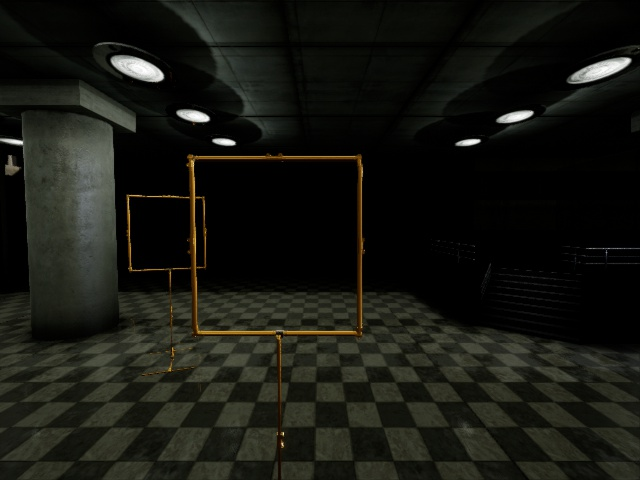
\includegraphics[width=\textwidth]{fig/gate_example}
		\caption{Original Image.}
		\label{fig:orig}
	\end{minipage}
	\begin{minipage}{0.33\textwidth}
		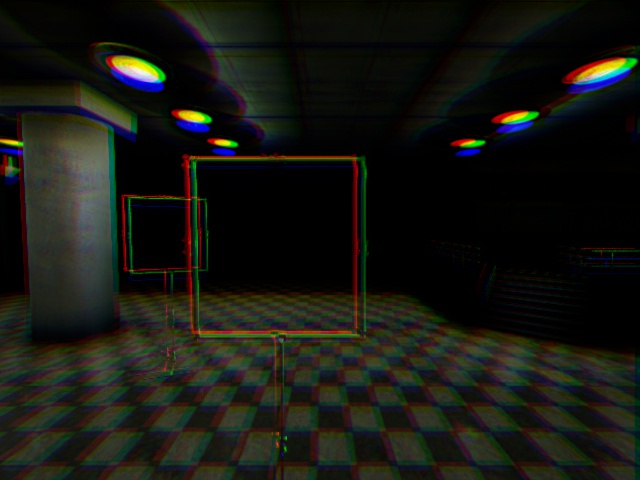
\includegraphics[width=\textwidth]{fig/gate_example_chromatic}
		\caption{Chromatic Aberration.} 		
		\label{fig:chromatic}
	\end{minipage}
	\begin{minipage}{0.33\textwidth}
		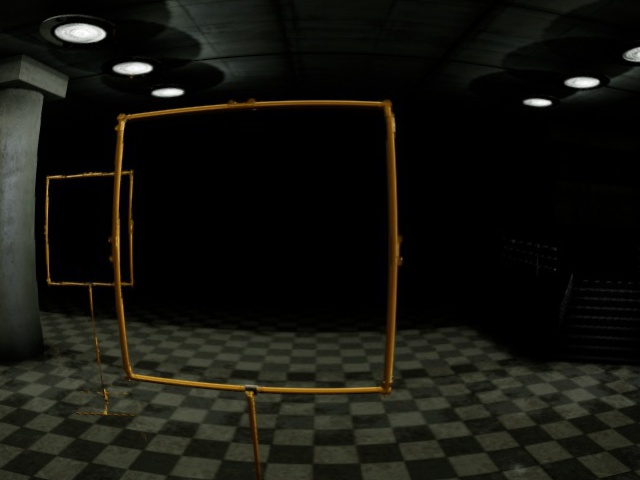
\includegraphics[width=\textwidth]{fig/gate_example_distorted}
		\caption{Lens Distortion. }		
		\label{fig:distortion}
	\end{minipage}
	
	\begin{minipage}{0.33\textwidth}
		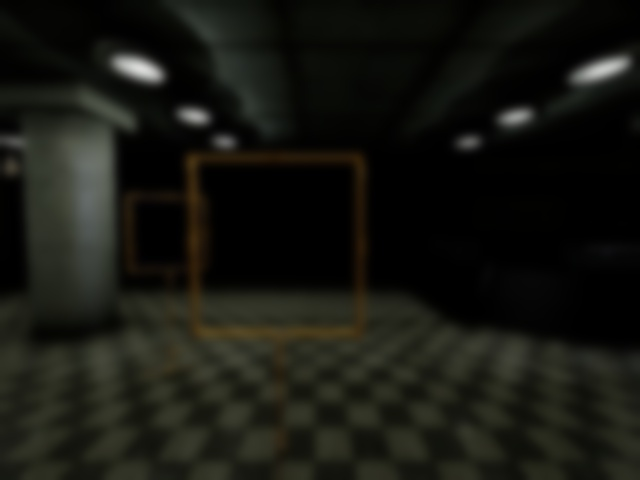
\includegraphics[width=\textwidth]{fig/gate_example_focusblur}
		\caption{Out-of-Focus blur.}
		\label{fig:focusblur}
	\end{minipage}
	\begin{minipage}{0.33\textwidth}
		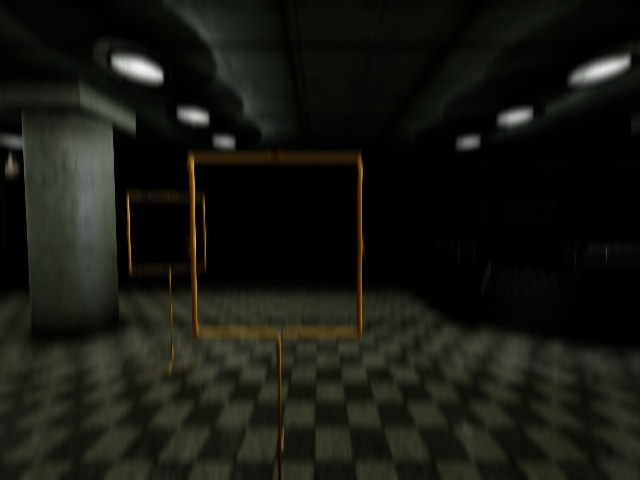
\includegraphics[width=\textwidth]{fig/gate_example_motionblur_v}
		\caption{Vertical Motion Blur.}
		\label{fig:motionblur}
	\end{minipage}
	\begin{minipage}{0.33\textwidth}
		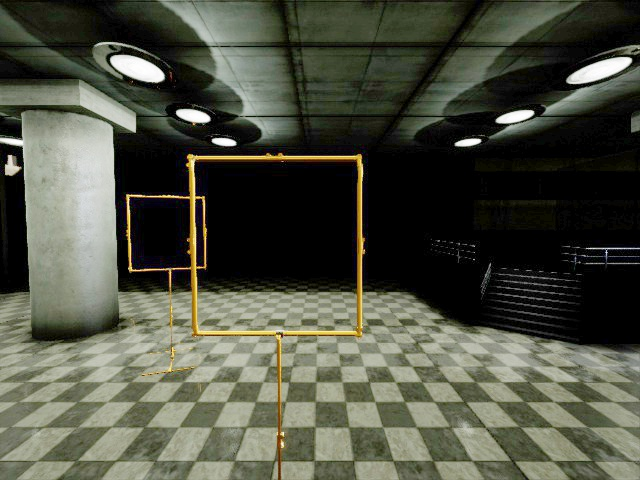
\includegraphics[width=\textwidth]{fig/gate_example_exposure}
		\caption{Exposure.}
		\label{fig:exposure}
	\end{minipage}
\end{figure}



\subsection{Experiments}
\todo{Distortion}
\subsection{Results}

\begin{figure}[htbp]
	\centering
	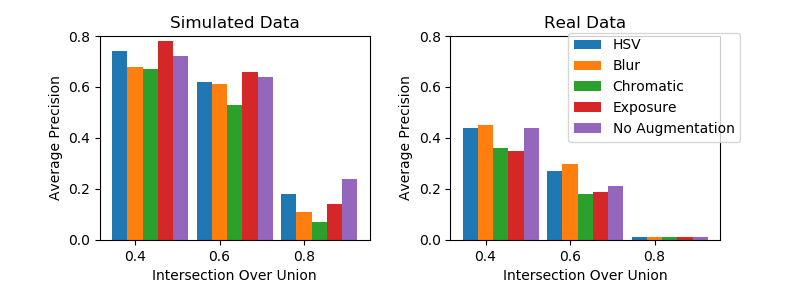
\includegraphics[width=\textwidth]{fig/pp_bar}
	\caption{Performance in terms of Average Precision for different methods  of image augmentation.}
	\label{fig:pp_bar}
\end{figure}

\Cref{fig:pp_bar} shows the results in terms of average precision in the training domain. On the simulated data variations in exposure improve the performance of low quality predictions slightly compared to using no augmentation. However, using no data augmentation achieves the best performance for high quality detections. The other effects have only minor influence. 

On the real data variations in HSV space as well as blurring improves the results compared to not using data augmentation. Incorporating chromatic aberration and variations in exposure lead to a deterioration in performance.

\subsection{Discussion}

In simulation the data augmentation has only a minor effect on low quality predictions, while the performance in high quality predictions decreases. As most effects are not really present in the test set this confirms that the models can learn a robust representation. Despite having more noise in the training data, the performance on the test set stays the same. However, the added noise leads to a lower quality in the predicted bounding boxes.

On the real data there is a stronger effect measurable. Variation in HSV and image blurring increase the performance compare to not using data augmentation. This meets our hypothesis that variations in HSV help to achieve a model that is more robust against changes in colour. Blur is one effect that can clearly be seen in the real world test set. Including this effect in the training process helped the model to perform better in the real world. Chromatic Aberration led to a significant improvement in \cite{Carlson2018} however, we cannot confirm these results. It is possible that our camera suffers only little from  chromatic aberration and thus including the effect in the training does not further help the prediction. The same holds for variations in exposure. 

\subsection{Conclusion}

We investigated whether including sensor effects present in the target domain in the data generation process can improve the detection. Therefore we modelled several effects that were observed when working with the camera or that improved the detection in experiments conducted in literature. Finally, image blurring improved the detection. Other effects led to a deterioration in performance.

We also investigated image augmentation by adding variations in HSV-space to evaluated whether this improves the robustness of the model, improving the performance on the real world dataset. We can confirm this hypothesis and conclude that this image augmentation should be part of the training process.

\section{Conclusion}
\label{sec:training:conclusion}

In this chapter the generation of data for the detection of \acp{EWFO} on \acp{MAV} was investigated. Finally, the initially formulated research questions can be answered:
\todo{put more numbers on the results}
\begin{enumerate}
	\item[\textbf{RQ1.1}] What role does context play for the detection \acp{EWFO} on \acp{MAV}?
	
	Without providing some variation in background, the trained model could not detect objects in simulation or the real world. However, when providing random images as background, the object could be detected sometimes. Hence, we conclude that at least some variation in background is required. Better results are obtained when the context is more realistic in terms of illumination and object placement even though when the environment is fully synthesized. Hence, we conclude that the model can make use of context and that creating a realistic synthesized environment is crucial for detection.
	
	\item[\textbf{RQ1.2}] What role does the view perspective play for the detection \acp{EWFO} on \acp{MAV}?
	
	We observe that the models perform poorer on objects with very low and very high distance. We assume that this is because less context is present and the object parts are spread over larger distances in the image.
	
	We could not identify a direct relation between the view perspective in training and during testing. Instead we see a trade-off in quality of bounding boxes in terms of detection and location and overall recall. The more angles are included in the training set the more objects can be detected however, more false positives are predicted and the dimensions of the bounding box are less accurate.
	
	\item[\textbf{RQ1.3}] Can the incorporation of sensor effects or image augmentation benefit the detection performance?
	
	Image blurring improved the performance of the models in the real world. We assume that  other effects are of minor influence in the camera used in this work. Thus modelling the respective effects did not help. In contrast motion blur seems to be of large influence. Incorporating this effect led to an improvement. Furthermore, we find that adding variations HSV-space improves the performance of the model in the real world.
	
\end{enumerate}


